The global transition toward a low-carbon economy is expected to significantly increase the demand for critical minerals required for renewable energy systems, electric vehicles, electricity grids, and energy storage technologies. Among these materials, copper occupies a particularly important position due to its excellent electrical and thermal conductivity. According to the International Energy Agency (IEA), electric vehicles require approximately 2.5 times more copper than conventional internal combustion vehicles \cite{IEA2021}. Renewable electricity infrastructures, battery storage systems, and modern power grids also rely heavily on copper-intensive technologies. As a result, several studies project a substantial increase in copper demand under global decarbonization scenarios \cite{Watari2020}.

However, this growing dependence on copper also creates an important environmental challenge. While copper is essential for electrification and renewable energy deployment, its extraction and processing remain highly energy-intensive activities requiring large quantities of fuel and electricity \cite{Norgate2010}. Consequently, the expansion of copper production may also increase greenhouse gas emissions and environmental pressures associated with mining activities.

\subsection{Chilean Context and Decarbonization Challenges}

Chile plays a central role in this global challenge as the world’s largest copper producer, accounting for more than 25\% of global copper production \cite{CochilcoWebsite2025}. The mining sector represents a fundamental component of the Chilean economy and contributes significantly to national exports, industrial activity, and public revenues. Copper extraction and processing therefore constitute both a major economic opportunity and an important environmental challenge for the country.

 \begin{figure}[H]
     \centering
     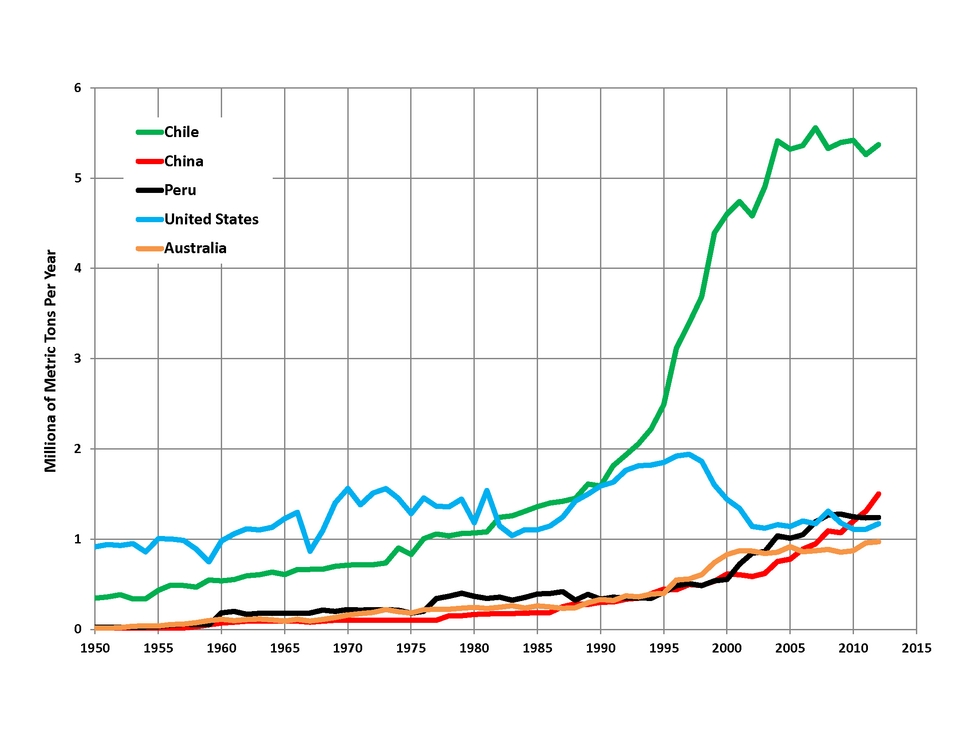
\includegraphics[width=0.8\linewidth]{Figures/image.png}
     \caption{Evolution of copper mine production in the world’s main producing countries between 1950 and 2015, measured in million metric tons per year. Chile experienced the most significant production growth over the period, consolidating its position as the world’s leading copper producer.}
     \label{fig:placeholder}
 \end{figure}

At the same time, Chile has established ambitious climate objectives aimed at achieving carbon neutrality by 2050 \cite{CAT2020}. Over the last decade, the country has rapidly expanded renewable electricity generation, particularly through solar and wind energy development. These transformations are especially relevant for the mining sector because electricity generation strongly influences the carbon footprint associated with copper production. As a result, the Chilean copper industry increasingly stands at the intersection between industrial development, resource extraction, and climate policy.

\subsection{Copper Production Chain and Scope of the Study}

Copper production involves several successive industrial stages that transform low-grade ore into high-purity metal. Depending on the ore type and extraction route, the production chain generally includes mining, crushing, grinding, concentration, smelting, refining, and electro-winning processes. These stages differ significantly in terms of energy requirements, fuel consumption, and electricity intensity.

Open-pit mining operations rely heavily on diesel-powered machinery for extraction and transportation activities, while mineral processing stages such as grinding, concentration, and electro-winning require large amounts of electricity. Smelting and refining operations are also particularly energy-intensive due to the high temperatures required for pyrometallurgical processes.

 \begin{figure}[H]
    \centering
    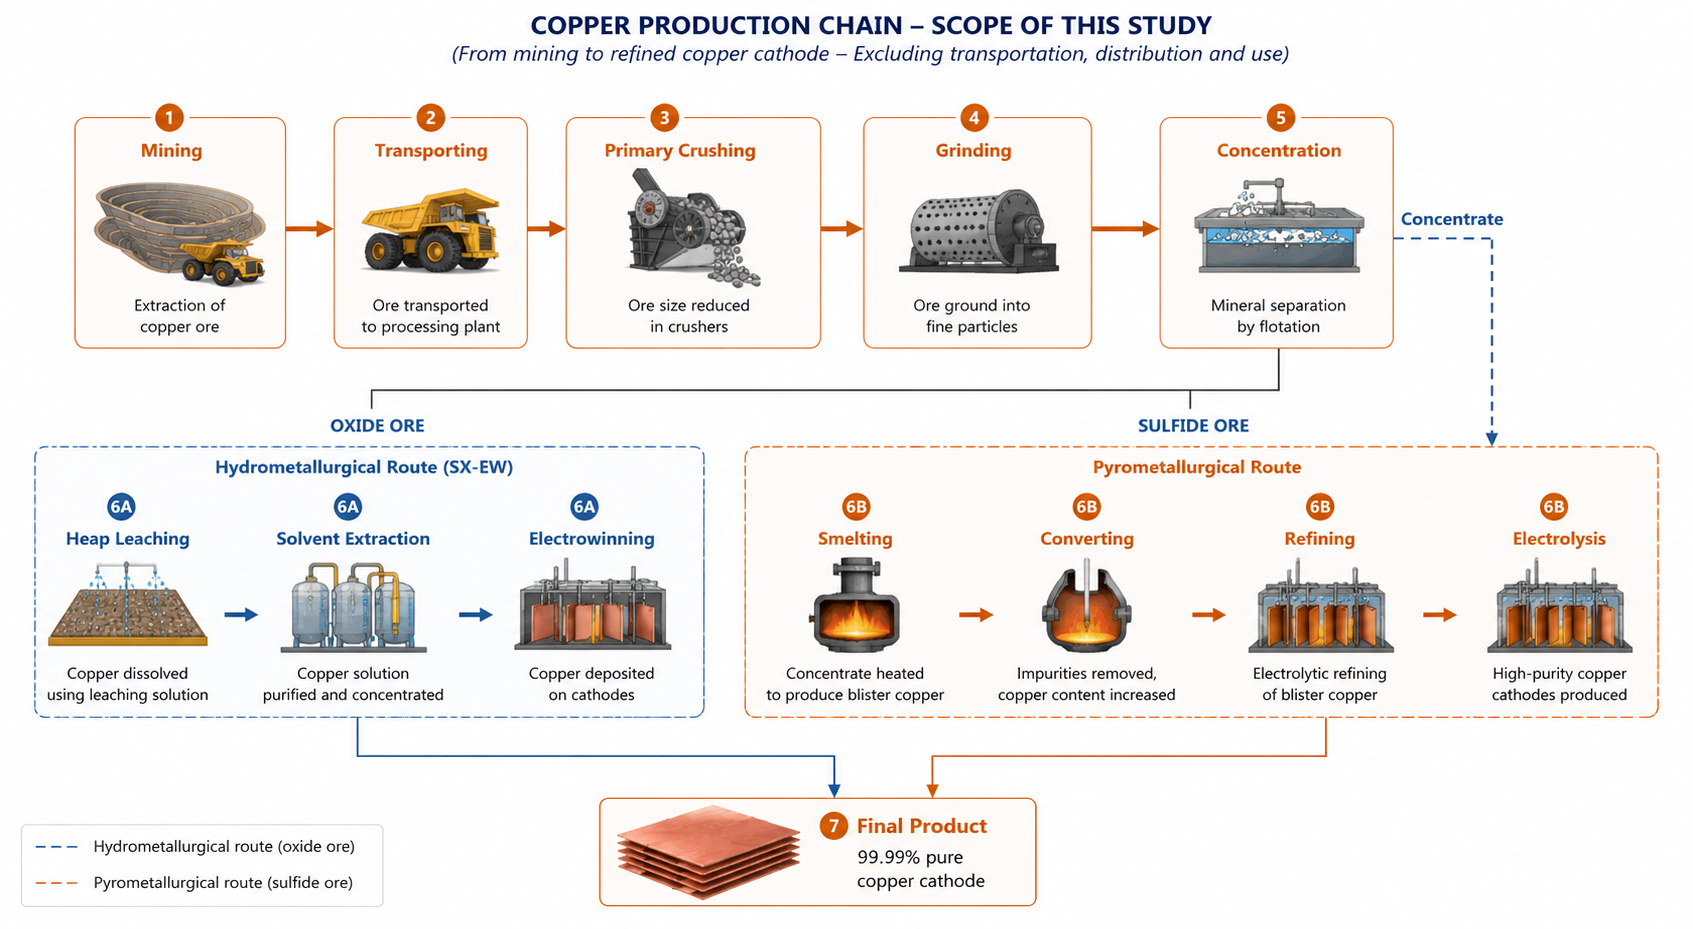
\includegraphics[width=1\linewidth]{Figures/Copper_production_chain_flowchart.png}
    \caption{Simplified representation of the copper production chain considered within the scope of this study. The figure illustrates the main industrial stages involved in transforming copper ore into 99.99\% pure copper cathodes through hydrometallurgical (SX-EW) and pyrometallurgical routes.}
    \label{fig:copper_process}
\end{figure}

Figure~\ref{fig:copper_process} illustrates the main stages of copper production considered within the scope of this study. Depending on the ore type, copper extraction follows either a hydrometallurgical route for oxide ores or a pyrometallurgical route for sulfide ores, both leading to the production of refined copper cathodes. The analysis focuses on the industrial extraction and processing chain, including mining, transportation within mining operations, crushing, concentration, smelting, refining, and electro-winning processes. Downstream stages such as commercialization, international transportation, manufacturing, product use, and end-of-life recycling are excluded from the system boundary. This scope allows the study to concentrate specifically on the industrial activities directly responsible for energy consumption and CO$_2$ emissions associated with copper production.

\subsection{Research Objectives and Methodological Approach}

Despite growing research on mining sustainability, understanding the evolution of CO$_2$ emissions in copper production remains challenging because emissions result from several interacting geological, technological, and energy-related factors. Existing studies often focus on specific aspects of mining decarbonization, such as renewable electricity integration or energy efficiency improvements, but fewer studies analyse how these different drivers jointly influence the evolution of emissions over time.

In this work, we analyse the evolution of CO$_2$ emissions in the Chilean copper mining industry using an IPAT-based decomposition framework. The study focuses on the respective roles of production growth, ore grade evolution, energy consumption, and the distinction between direct emissions from fuel combustion and indirect emissions associated with electricity use. The analysis relies on industrial datasets published by the Chilean Copper Commission (Cochilco), including production, ore grades, energy consumption, and greenhouse gas emissions by process type.

\subsection{Research Questions}

This report aims to answer the following questions:

\begin{itemize}
    \item How have CO$_2$ emissions associated with Chilean copper production evolved over time?

    \item To what extent have production growth, ore grade decline, energy consumption and carbon intensity influenced these emissions?

    \item How can electrification and the decarbonization of Chile’s electricity system contribute to reducing the environmental impact of copper production?
\end{itemize}

% Copper has become one of the most strategic materials in the global effort to reduce greenhouse gas emissions and transition toward a low-carbon economy. Due to its excellent electrical and thermal conductivity, copper is essential for renewable energy technologies, electric vehicles, electrical grids, and energy storage systems. Nevertheless, the extraction and processing of copper require large amounts of energy, making the industry itself a significant source of CO$_2$ emissions. This creates an important contradiction: while copper is indispensable for decarbonization, its production contributes to environmental pollution.

% A central actor in this global challenge is Chile, a South American country that possesses the world’s largest copper reserves and remains the leading producer of copper worldwide. Chile alone accounts for approximately 20\% of global copper reserves and contributes more than 27\% of world copper production. The mining sector is therefore fundamental to the Chilean economy, generating a substantial share of national GDP, exports, and public income. However, the environmental impact of this activity is considerable. Copper extraction in Chile is highly energy-intensive, particularly because ore grades have progressively declined and mining operations have expanded to greater depths. Consequently, mining activities generate significant greenhouse gas emissions. At the same time, Chile benefits from exceptional renewable energy potential, especially in solar and wind energy, which could support the decarbonization of mining operations in the future.

% In this work, we analyse the main drivers of CO$_2$ emissions in the Chilean copper mining industry using an IPAT-based decomposition framework. The study aims to distinguish the relative influence of production growth, ore grade decline, energy intensity, fuel consumption, and electricity-related emissions on the evolution of total greenhouse gas emissions. Particular attention is given to the separation between direct emissions from fuel combustion and indirect emissions associated with electricity use. The analysis focuses on the Chilean copper extraction and processing sector and relies on industrial data published by the Chilean Copper Commission (Cochilco), including production, ore grades, energy consumption, and greenhouse gas emissions by process type.

% \vspace{1em}
% \vspace{1em}
% \subsection{The importance of Copper extraction for Chile's economy}

% Chile has established many climate objectives aimed at helping the global transition toward a low-carbon economy while also addressing the environmental impacts associated with its resource-intensive industries, particularly industries such as mining and copper production. According to the Climate Action Tracker(put ref), Chile’s updated Nationally Determined Contribution (NDC) commits the country to limiting greenhouse gas emissions to a maximum of 95 MtCO$_2$e by 2030 and maintaining a cumulative emissions budget of no more than 1,100 MtCO$_2$e for the 2020–2030 period. The country also plans to ensure that national emissions peak no later than 2025, after which a gradual reduction trajectory should begin. In the longer term, Chile has legally committed, through its Climate Change Framework Law, to achieving carbon neutrality by 2050. To accomplish these goals, Chile is focusing heavily on expanding renewable energy generation, especially solar and wind power, which are particularly important given the country’s exceptional natural resources in the Atacama Desert and coastal regions. The government is also pursuing the gradual phase-out of coal-fired power plants ( a reformuler) , promoting electrification and electromobility, increasing energy efficiency across industrial sectors, and strengthening climate resilience and adaptation measures. Forest conservation and reforestation policies are another central component of Chile’s strategy because natural carbon sinks (plus de details?) are expected to play a major role in offsetting emissions. Furthermore, Chile aims to modernize its mining sector by encouraging cleaner production methods, improving water management, reducing transportation emissions, and increasing the use of renewable electricity in copper extraction and refining processes. These goals are especially significant because Chile is the world’s largest copper producer, and copper is essential for renewable technologies such as electric vehicles, batteries, wind turbines, and power grids. The Climate Action Tracker evaluates Chile’s climate targets as “Almost sufficient,” meaning that while the country has made important progress and its policies are relatively ambitious compared to many nations, additional measures and stronger emission reductions are still necessary for full alignment with the Paris Agreement’s objective of limiting global warming to 1.5°C.
%  \begin{figure}[H]
%     \centering
%     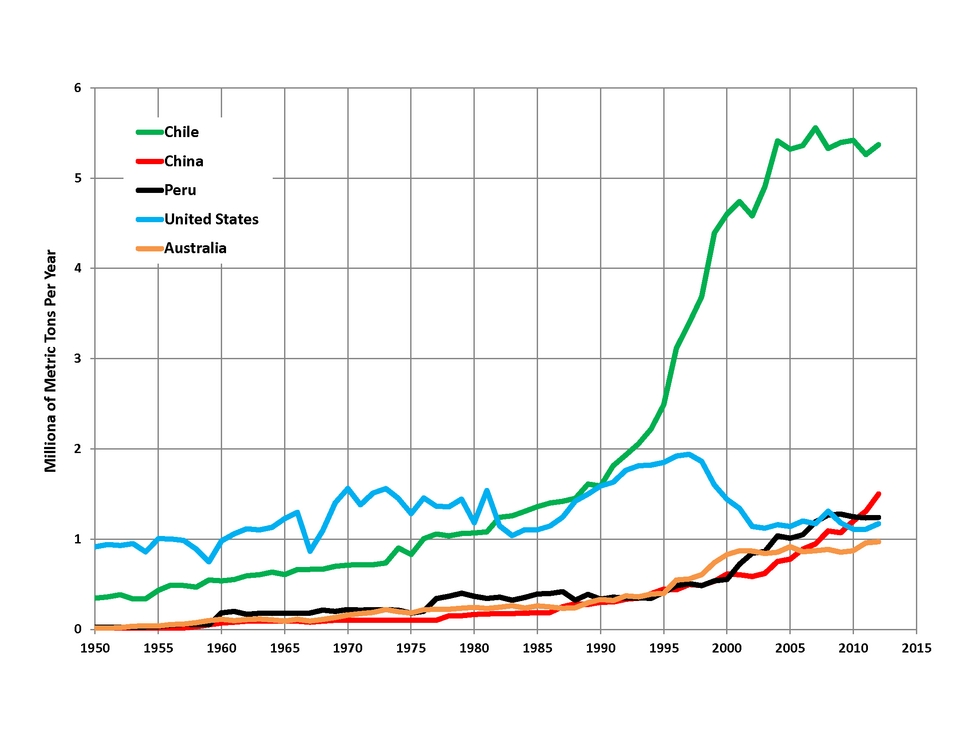
\includegraphics[width=0.5\linewidth]{Figures/image.png}
%     \caption{Wikipedia source}
%     \label{fig:placeholder}
% \end{figure}

% \vspace{1em}
% \vspace{1em}
% \subsection{Production Chain of Copper}

% The extraction of copper in Chile involves several key stages that transform low-grade ore into high-purity metal. It begins with \textbf{mining}, mainly through open-pit operations, where large quantities of rock containing less than 1\% copper are excavated. The ore is then crushed and processed in the \textbf{concentration} stage, where physical and chemical methods separate copper minerals to produce a concentrate containing about 25--35\% copper. This concentrate undergoes \textbf{smelting and refining}, where heat and chemical processes remove impurities, followed by \textbf{electrolysis} to achieve very high purity (up to 99.99\%). Finally, the refined copper is shaped during \textbf{final processing} into products such as wires, sheets, and alloys used in various industries. Together, these stages form a complex and resource-intensive process that is essential for supplying copper to global markets \cite{CNEP2025}.

% Copper mining in Chile is dominated by large-scale open-pit mines because many copper deposits are located close to the surface and extend over vast geographical areas. These mining operations require heavy machinery such as drills, excavators, loaders, and haul trucks to remove enormous quantities of waste rock and ore. In some cases, underground mining methods are also employed when ore bodies are located at greater depths. Once extracted, the ore is transported to nearby beneficiation plants where crushing and grinding operations reduce the material into fine particles to facilitate mineral separation.

% The concentration stage generally relies on flotation techniques, where chemical reagents and air bubbles are introduced into the crushed ore slurry to selectively separate copper-bearing minerals from waste material. The resulting copper concentrate contains significantly higher copper content and can then be economically transported to smelting facilities. Smelting represents one of the most energy-intensive stages of the production chain because the concentrate must be heated at extremely high temperatures to separate metallic copper from sulfur and other impurities. This process produces blister copper, which is then further purified during electrolytic refining to obtain cathode copper with purity levels suitable for industrial and electrical applications.

% In parallel to the traditional pyrometallurgical route, certain low-grade or oxide ores are processed using hydrometallurgical techniques such as \textbf{leaching-solvent extraction-electrowinning (LX-SX-EW)}. In this process, acidic solutions dissolve copper directly from the ore, after which solvent extraction purifies and concentrates the solution before electrowinning recovers pure copper metal. Compared to conventional smelting, this method generally requires lower temperatures and can be more suitable for specific ore types.

% The copper production chain also depends heavily on supporting infrastructure and industrial services. Transportation systems, electricity supply, water management facilities, tailings storage, and waste treatment operations are all necessary to maintain continuous production. Because many mining regions in Chile are located in arid areas such as the Atacama Desert, water supply and energy availability represent major operational challenges. Consequently, mining companies are increasingly investing in renewable energy systems, desalination plants, and more efficient technologies to reduce both operational costs and environmental impacts.

% Overall, the copper production chain combines highly advanced industrial processes with large-scale infrastructure and energy consumption. While these processes are essential for supplying global demand for copper, they also contribute significantly to greenhouse gas emissions and environmental pressures, making the modernization and decarbonization of the sector a major priority for Chile and the global mining industry.

% \cite{CNEP2025}.

% \subsection{Copper Extraction Process}

% The production of copper involves a sequence of interconnected industrial processes that transform raw ore into high-purity metal. These processes can be broadly divided into mining, beneficiation, smelting, refining, and hydrometallurgical treatment, each playing a critical role in the overall value chain.

% The process begins with \textbf{mining}, which can be performed using either open-pit or underground methods depending on the depth and geology of the ore deposit. Open-pit mining is the most common method, involving large-scale excavation of surface material in stepped benches, while underground mining uses shafts and tunnels to access deeper ore bodies. Both methods require heavy machinery and extensive infrastructure to extract and transport the ore to processing facilities.

% Once extracted, the ore undergoes \textbf{beneficiation}, also known as ore dressing or concentration. This stage involves crushing and grinding the ore into fine particles to liberate copper minerals from the surrounding rock. The material is then processed using flotation, a technique in which chemical reagents and air bubbles are introduced to selectively separate copper minerals. The result is a copper concentrate containing approximately 25--40\% copper, significantly increasing its economic value.

% The concentrated material is then sent to a \textbf{smelter}, where pyrometallurgical processes are used. In this high-temperature stage, the concentrate is heated in furnaces to remove impurities and separate metal from waste material (slag). This produces \textit{blister copper}, which typically contains around 98--99\% copper. Smelting is energy-intensive and contributes significantly to the overall emissions of the copper production chain.

% Following smelting, the copper undergoes \textbf{electrolytic refining}. In this process, copper anodes are dissolved in an electrolyte solution, and pure copper is deposited onto cathodes using an electric current. This electrochemical process removes remaining impurities and produces copper with a purity of up to 99.99\%, suitable for electrical and industrial applications.

% In parallel to the pyrometallurgical route, low-grade or oxide ores are often processed using a hydrometallurgical method known as \textbf{leaching-solvent extraction-electrowinning (LX-SX-EW)}. In this process, copper is first dissolved from the ore using acidic solutions (leaching). The solution is then purified and concentrated through solvent extraction (SX), and finally, copper is recovered as solid metal through electrowinning (EW). This method is particularly efficient for lower-grade ores and has lower energy requirements compared to traditional smelting.

% Finally, \textbf{production services} support all stages of copper extraction. These include material handling systems, transportation (trucks, conveyors), energy supply, water management, and waste treatment such as tailings storage. These supporting systems are essential for maintaining continuous and efficient operations throughout the entire process.

% In conclusion, copper production is a complex and resource-intensive process involving multiple stages that progressively increase the metal's purity and value. Both pyrometallurgical and hydrometallurgical routes are used depending on ore type, and modern operations rely heavily on advanced technologies and infrastructure to optimize efficiency and reduce environmental impact. 

% \subsection{Possible Main Drivers of CO$_2$ Emissions in Copper Extraction} 


% The main drivers of CO$_2$ emissions in copper extraction are associated with the high energy intensity and complexity of the production chain. A major source of emissions comes from \textbf{mining operations}, where diesel-powered machinery is used for drilling, blasting, and transporting large volumes of ore. Significant emissions also arise during \textbf{crushing and grinding} in the beneficiation stage, which require substantial electricity. The \textbf{smelting and refining} phases are particularly carbon-intensive due to the need for high-temperature furnaces, often powered by fossil fuels. In addition, \textbf{transportation} of ore, concentrate, and refined copper across long distances contributes to indirect emissions. The reliance on fossil-based energy for electricity generation further increases the overall carbon footprint. Finally, \textbf{waste management and tailings processing} can also contribute to emissions, especially when involving additional energy use and chemical treatments. Together, these factors make copper extraction a resource- and energy-intensive process with significant environmental impacts.

% \vspace{1em}


% \vspace{1em}
% \subsection{Copper as a Means to Reduce CO$_2$ Emissions}

% Copper is considered one of the most important strategic materials in the global transition toward a low-carbon economy because of its exceptional electrical and thermal conductivity. These physical properties make copper indispensable for the development, transmission, and efficient use of electricity in modern energy systems. As countries seek to reduce their dependence on fossil fuels and increase the share of renewable energy in their energy mix, the demand for copper continues to rise significantly. Renewable technologies such as solar photovoltaic panels, wind turbines, hydroelectric systems, and battery storage installations require substantially larger quantities of copper compared to conventional fossil-fuel-based technologies. This is mainly due to the need for efficient electrical connections, power conversion systems, generators, transformers, and transmission cables.

% Copper also plays a fundamental role in the electrification of transportation, which is considered one of the key solutions for reducing greenhouse gas emissions worldwide. Electric vehicles (EVs), including cars, buses, and rail systems, require considerably more copper than traditional internal combustion engine vehicles. Copper is extensively used in electric motors, batteries, inverters, charging stations, and onboard electrical systems because it enables efficient energy transfer and minimizes energy losses. In addition, the expansion of charging infrastructure and smart electricity grids further increases the importance of copper in supporting sustainable transportation systems. By facilitating the replacement of fossil-fuel-powered transport with electric alternatives, copper contributes directly to the reduction of CO$_2$ emissions associated with mobility and urban transportation.

% Beyond transportation and renewable electricity generation, copper is also essential for improving energy efficiency across industrial, residential, and commercial sectors. Efficient electrical systems reduce energy losses during transmission and distribution, thereby lowering the total amount of energy required for economic activities. Modern power grids, energy storage technologies, and advanced electronic systems all rely heavily on copper components to ensure reliable and efficient operation. Consequently, copper indirectly contributes to reducing global emissions by enhancing the overall efficiency of energy systems and enabling the integration of intermittent renewable energy sources into national electricity networks.

% Another major environmental advantage of copper lies in its recyclability. Copper can be recycled an unlimited number of times without losing its chemical or physical properties, making it highly suitable for circular economy strategies. Recycling copper requires significantly less energy than primary extraction and refining, which substantially reduces greenhouse gas emissions and decreases the environmental impact associated with mining activities. Secondary copper production therefore plays a crucial role in limiting the demand for newly mined copper while supporting sustainable resource management. Today, recycled copper already represents an important share of global copper production and is expected to become increasingly significant as demand for clean technologies continues to expand.

% Nevertheless, despite its positive contribution to decarbonization, copper production itself remains energy-intensive and can generate substantial CO$_2$ emissions. Mining operations, ore transportation, smelting, and refining processes often rely on fossil fuels and large amounts of electricity. This creates an important paradox in the energy transition: copper is essential for reducing emissions globally, yet its extraction and processing can contribute significantly to environmental pollution if not managed sustainably. For this reason, many countries, including Chile, are investing in cleaner mining technologies, renewable energy integration, and more efficient refining processes to reduce the carbon footprint of copper production.

% As global efforts to combat climate change intensify, copper is expected to remain at the center of decarbonization strategies. The growing deployment of renewable energy systems, electric vehicles, energy storage technologies, and electrified infrastructure will continue to increase copper demand in the coming decades. Consequently, ensuring a sustainable and low-carbon copper supply chain has become a critical challenge for governments, industries, and policymakers worldwide.


% \subsection{CO$_2$ Emissions Reduction in Chile}
% In 2020, Chile announced two targets for emissions reduction. The first, due in 2030, aims for an unconditional absolute target of 95~MtCO$_2$e or a cumulative emissions budget of 1{,}100~MtCO$_2$e, as well as a conditional emissions reduction target of up to 45\% net greenhouse gas (GHG) emissions reduction, subject to specific financial, market, technological, and political conditions \cite{CATChile2020}.

% Chile has made significant progress in reducing CO2 emissions through various initiatives and policies in the past few years.  

% \begin{figure}[H]
%     \centering
%     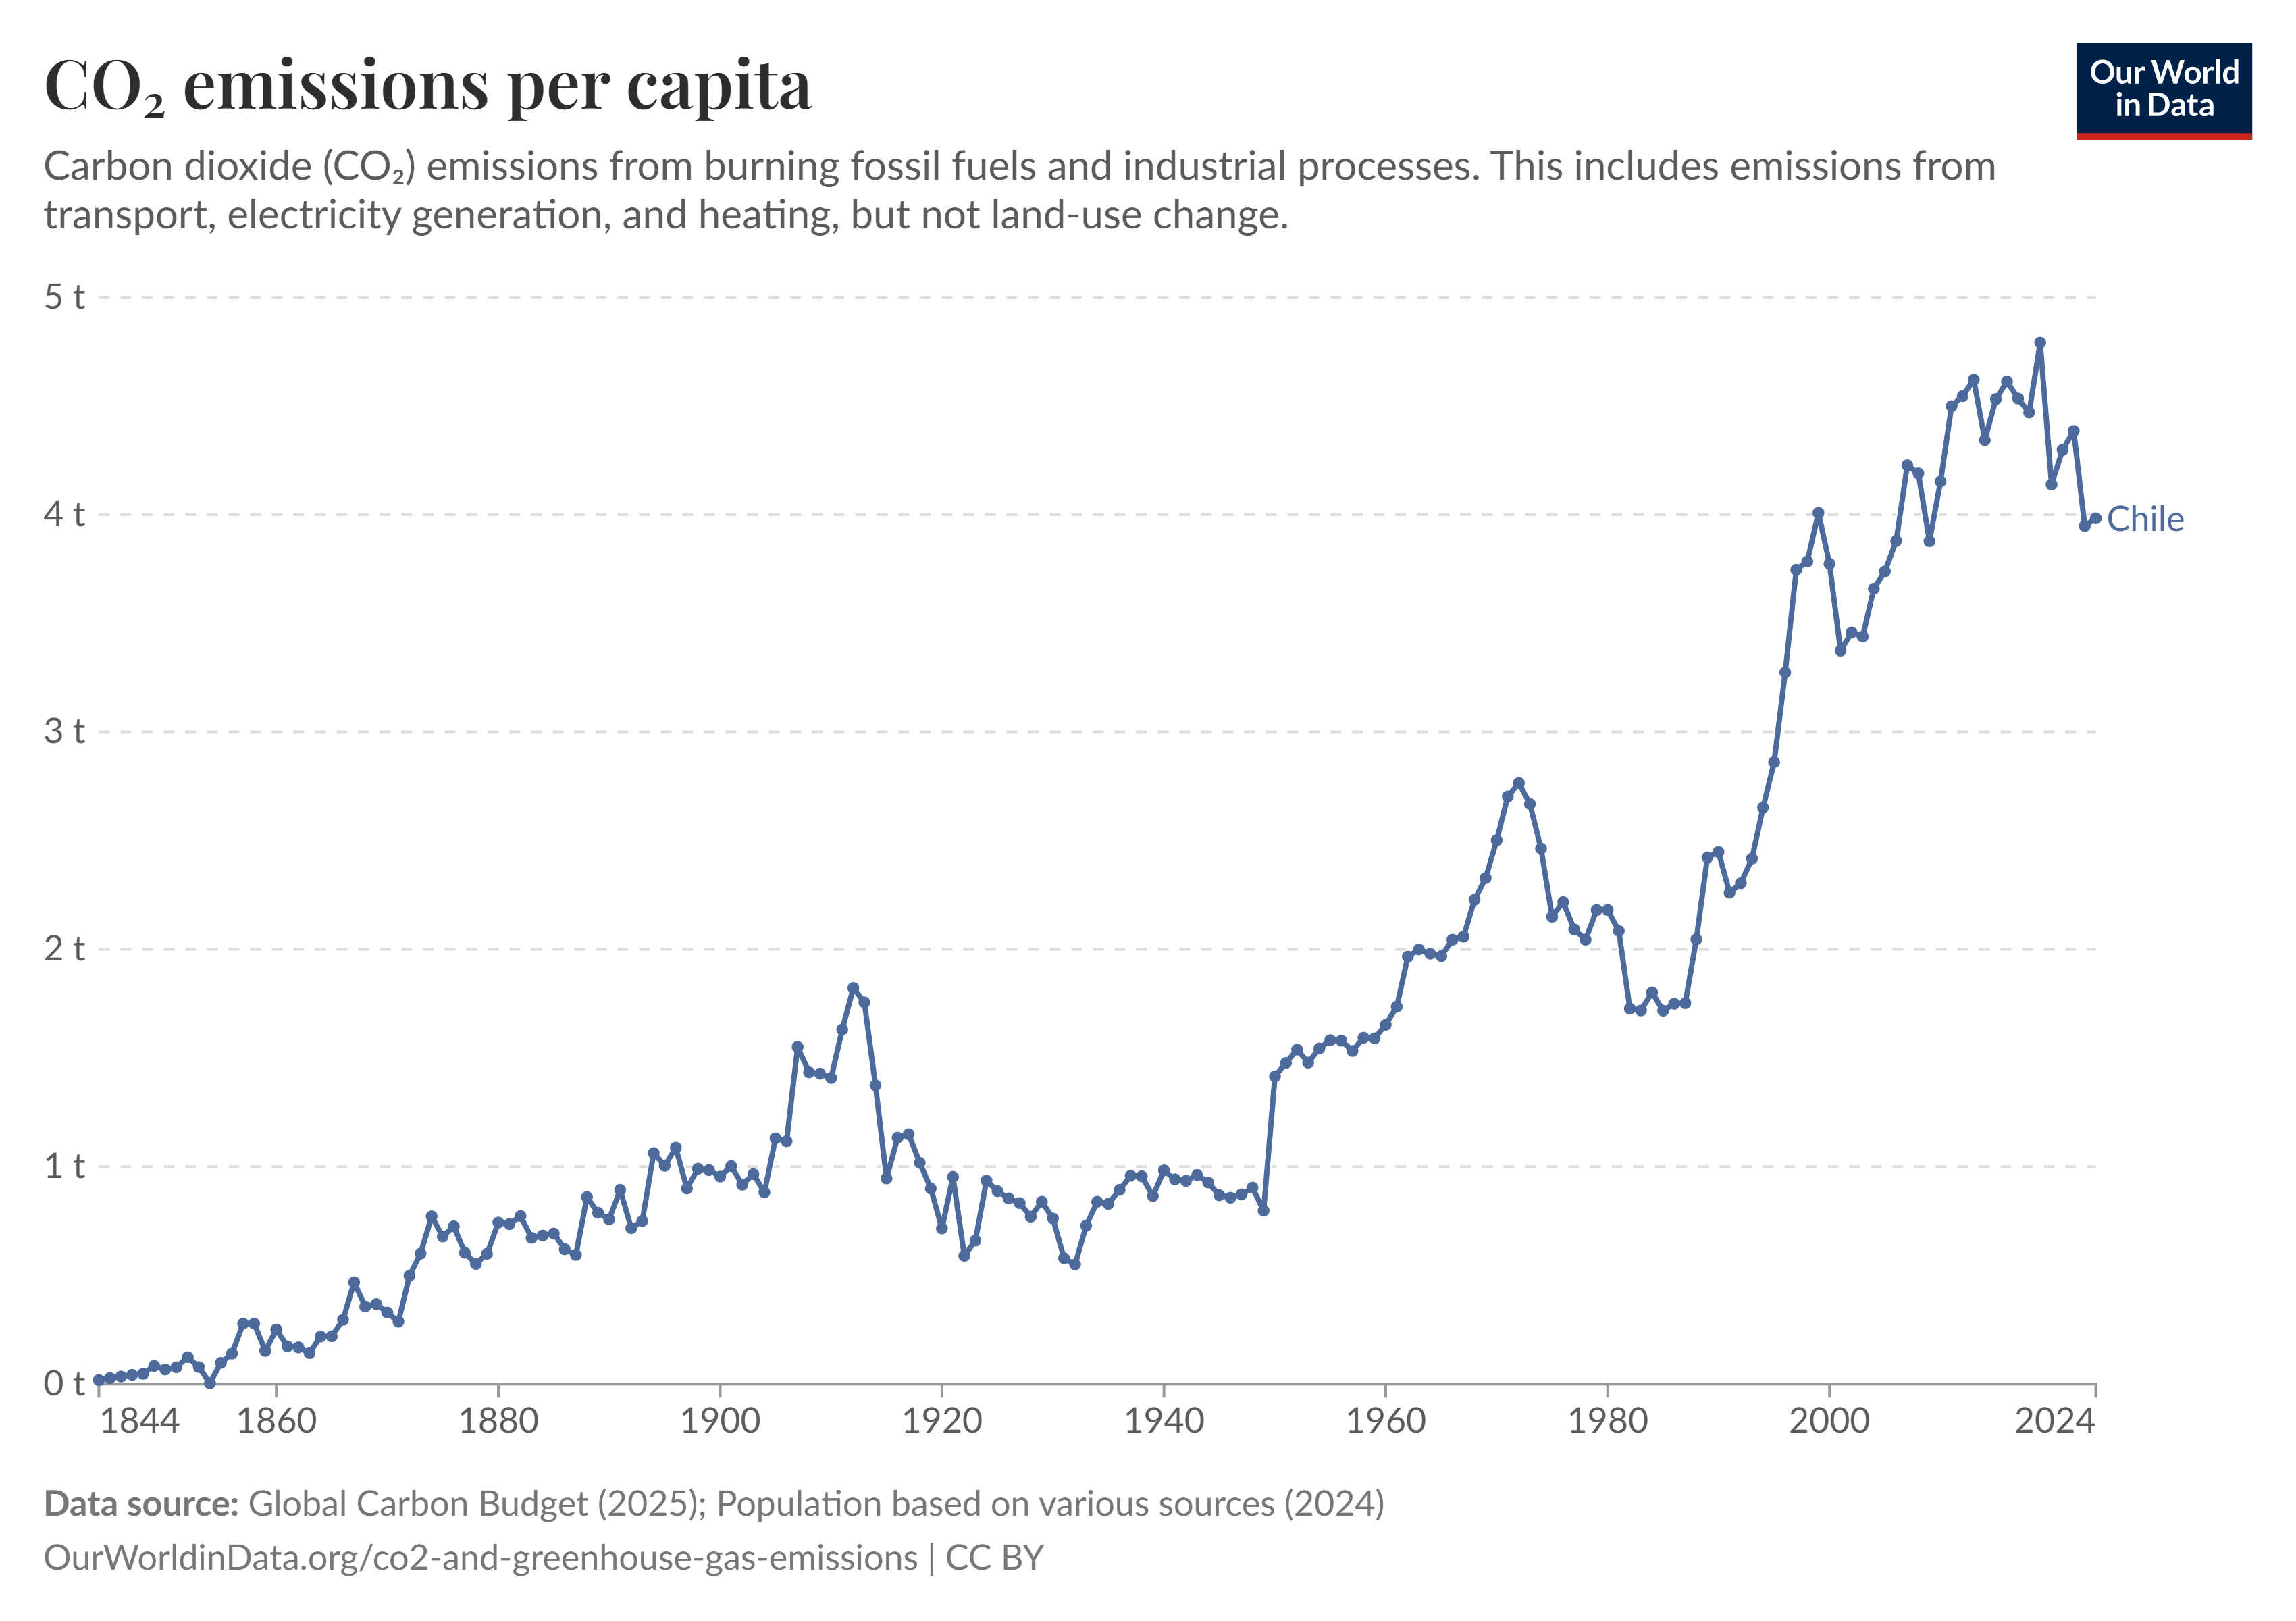
\includegraphics[width=0.5\linewidth]{Figures/co-emissions-per-capita (1).png}
%     \caption{Enter Caption}
%     \label{fig:placeholder}
% \end{figure}



% https://greeniron.se/visit-in-chile-one-of-the-worlds-leading-mining-countries/?
% \vspace{1em}
% Global Journal of Flexible Systems Management (December 2025) 26(4):813–837
% https://doi.org/10.1007/s40171-025-00464-w